% Official AIP / J. Chem. Phys. class options (REVTeX 4.2).
% Template: aiptemplate.tex / aipsamp.tex in the REVTeX distribution
%   https://journals.aps.org/revtex/
%   \documentclass[aip,jcp,reprint,amsmath,amssymb]{revtex4-2}
% Use "preprint" instead of "reprint" for the 12 pt, single-column
% double-spaced review copy requested by AIP Peer X-Press.
\documentclass[%
 aip,
 jcp,
 amsmath,amssymb,
 reprint,
 floatfix,
]{revtex4-2}

\usepackage{graphicx}
\usepackage{dcolumn}
\usepackage{bm}
\usepackage{booktabs}
\usepackage{hyperref}

\newtheorem{theorem}{Theorem}
\newtheorem{corollary}{Corollary}
\newtheorem{proposition}{Proposition}
\newtheorem{remark}{Remark}

\newcommand{\avg}[1]{\langle #1 \rangle}
\newcommand{\xip}{\bar{\xi}_p}
\newcommand{\chip}{\chi_p}
\newcommand{\kB}{k_{\mathrm{B}}}
\newcommand{\kQRR}{k_{\mathrm{QRR}}}
\newcommand{\kQTST}{k_{\mathrm{QTST}}}
\newcommand{\kTST}{k_{\mathrm{TST}}}

\begin{document}

\preprint{AIP/123-QED}

\title[Path-spread-resolved QTST]{Path-spread-resolved quantum transition-state theory for proton transfer}

\author{Mercel Vubangsi}
\email{m.vubangsi@miu.edu}
\affiliation{Department of Physics, Maharishi International University, Fairfield, Iowa 52557, USA}
\affiliation{Research Center for AI and IoT, Near East University, Nicosia 99138, Cyprus}
\affiliation{Department of Physics, University of Bamenda, Bambili, Cameroon}

\author{Fadi Al-Turjman}
\affiliation{Research Center for AI and IoT, Near East University, Nicosia 99138, Cyprus}

\author{Martin Tchoffo}
\affiliation{Department of Physics, University of Dschang, Dschang, Cameroon}

\date{\today}

\begin{abstract}
Centroid quantum transition-state theory and ring-polymer molecular dynamics yield thermal rates, but they collapse the imaginary-time path of the transferring proton onto a single collective coordinate. We define the proton-path spread $\chip$ as the mean-square bead displacement of the ring polymer along the proton-sharing coordinate---the squared radius of gyration projected onto that coordinate---and use it to resolve the centroid dividing-surface ensemble by imaginary-time geometry. The associated path-spread-resolved (QRR) formula is a decomposition of the usual centroid flux, not a more accurate dynamical rate. For a harmonic proton mode, $\avg{\chip}$ has a closed continuum formula and an exact finite-bead counterpart; Levy-staging path-integral Monte Carlo reproduces the finite-bead result to within $1\%$. The H/D ratio of $\avg{\chip}$ interpolates between $\sqrt{m_D/m_H}$ as $T\to 0$ and $m_D/m_H$ as $T\to\infty$. Exact Eckart rates at $300\,\mathrm{K}$ give a tunneling correction $\kappa_H=1.28$--$2.68$ and a kinetic isotope effect of $1.68$--$2.28$ as the barrier rises from $4$ to $16\,\kB T$, against a classical isotope factor of $\sqrt{2}$. On an asymmetric double well, umbrella sampling shows that the dividing-surface path-spread distribution for H is systematically broader than for D ($f_{\mathrm{deloc}}^{\mathrm{H}}\approx 0.18$--$0.23$ versus $f_{\mathrm{deloc}}^{\mathrm{D}}\approx 0.01$--$0.04$). We do not report a QRR rate, nor a condensed-phase application. The estimator is a collective variable that can be accumulated in any existing path-integral code.
\end{abstract}

\keywords{proton transfer, path-integral molecular dynamics, quantum transition-state theory, kinetic isotope effect, ring-polymer molecular dynamics}

\maketitle

\section{Introduction}

Proton transfer, and proton-coupled electron transfer (PCET) in particular, is a setting in which nuclear quantum effects, solvent reorganization, and, at electrodes, the applied potential jointly control the rate.\cite{hammes-schiffer2015,soudackov2000,marcus1956,klinman2013} Kinetic isotope effects (KIEs) and non-Arrhenius temperature dependence are the usual experimental signatures of tunneling,\cite{westheimer1961,klinman2013} but they do not by themselves identify the imaginary-time path geometry that carries the reactive flux.

Path-integral methods address that geometry at the level of the thermal density matrix.\cite{feynman1948,feynman1965,chandler1981} Centroid quantum transition-state theory (QTST) replaces the classical reaction coordinate by the ring-polymer centroid and evaluates a flux through a dividing surface in centroid space.\cite{voth1989,cao1994,gillan1987,hele2013} Ring-polymer molecular dynamics (RPMD) propagates the same polymer in real time and supplies a recrossing correction to the centroid flux.\cite{craig2004,craig2005,habershon2013} Instanton theory, in the complementary deep-tunneling limit, optimizes a single dominant imaginary-time orbit.\cite{richardson2009,richardson2018} Transition-path sampling retains full real-time path information, at a cost that is not organized by equilibrium imaginary-time geometry.\cite{bolhuis2002}

What these approaches do not provide is a cheap, equilibrium order parameter that distinguishes compact ring polymers (thermally activated, localized near the donor or acceptor) from delocalized polymers whose beads span the transfer coordinate (tunneling-like imaginary-time geometry). The ring-polymer radius of gyration is already used as a diagnostic of delocalization in condensed-phase proton studies.\cite{drechsel2014,marsalek2017} Here we restrict that diagnostic to the chemical sharing coordinate, give it exact harmonic limits, and use it to \emph{condition} the QTST flux.

The resulting path-spread-resolved rate, which we call QRR, is
\begin{equation}
  \kQRR
  =
  \int_0^\infty d\chip\;
  \kQTST(\chip)\,
  \kappa(\chip)\,
  p^\ddagger(\chip),
  \label{eq:kQRR}
\end{equation}
where $p^\ddagger(\chip)$ is the distribution of path spreads at the dividing surface and $\kappa(\chip)$ is a class-conditional transmission coefficient. When $\kappa$ is taken independent of $\chip$, Eq.~\eqref{eq:kQRR} reduces identically to ordinary QTST. QRR is therefore a decomposition of a known estimator, not a claim of a more accurate thermal rate. Its value is mechanistic: it reports which imaginary-time geometries carry the flux, how that mix depends on isotope and barrier, and whether path spread couples to a solvent coordinate.

Section~\ref{sec:theory} defines $\chip$ and the conditional free energy, states the solvable limits, and writes the flux decomposition. Section~\ref{sec:methods} describes the samplers. Section~\ref{sec:results} reports harmonic, Eckart, and double-well calculations. Section~\ref{sec:discussion} discusses scope and limitations. We do not report condensed-phase electrochemical simulations; those require a validated reactive potential and are left as an application of the estimator.

\section{Theory}
\label{sec:theory}

\subsection{Path-spread functional}

The $P$-bead ring-polymer representation of the canonical density is standard.\cite{chandler1981,cao1994} For a proton transferring between donor and acceptor oxygens we use the bead-resolved sharing coordinate
\begin{equation}
  \xi_p^{(s)} = r_{\mathrm{ODH}}^{(s)} - r_{\mathrm{OAH}}^{(s)},
  \qquad
  \xip = P^{-1}\sum_{s=1}^{P}\xi_p^{(s)}.
\end{equation}
The path-spread functional is the bead variance along that coordinate,
\begin{equation}
  \chip
  =
  \frac{1}{P}\sum_{s=1}^{P}
  \bigl(\xi_p^{(s)}-\xip\bigr)^2.
  \label{eq:chip}
\end{equation}
This is the squared radius of gyration of the polymer projected onto $\xi_p$. It is identically zero at $P=1$ and is non-negative for all configurations. Compact paths have $\chip$ of order the zero-point spread in a well; delocalized paths have $\chip$ large enough that beads occupy both sides of the barrier.

The joint density $P(\xip,\chip)$ defines the conditional free energy
\begin{equation}
  F(\xip,\chip) = -\kB T\ln P(\xip,\chip)+C.
  \label{eq:F}
\end{equation}
Projection onto $\xip$ recovers the centroid potential of mean force.\cite{cao1994} Slices at fixed $\xip$ resolve path class, as sketched in Fig.~\ref{fig:schematic}. A solvent or energy-gap coordinate $\lambda_s$ may be added without changing the construction; the three-dimensional surface $F(\xip,\chip,\lambda_s)$ is the natural object for PCET, but the calculations below are two-dimensional unless stated.

\begin{figure*}[t]
\centering
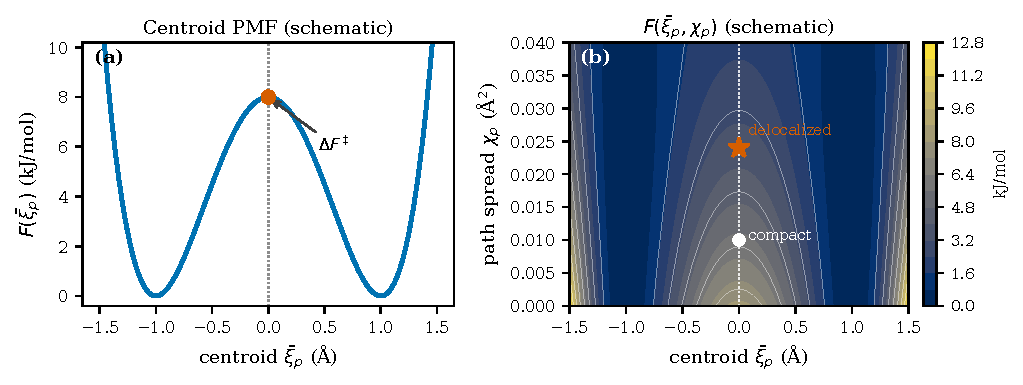
\includegraphics[width=0.95\textwidth]{../figures/fig1_schematic.pdf}
\caption{\label{fig:schematic}
Schematic, not computed data.
(a)~Centroid potential of mean force $F(\xip)$, in which all ring-polymer shapes at a given centroid are averaged.
(b)~Conditional free energy $F(\xip,\chip)$. Compact and delocalized dividing-surface geometries that share $\xip=0$ are marked.
}
\end{figure*}

\subsection{Flux decomposition}
\label{sec:flux}

Let $\xip^\ddagger$ locate the dividing surface. The marginal
\begin{equation}
  p^\ddagger(\chip)
  =
  \frac
  {e^{-\beta F(\xip^\ddagger,\chip)}}
  {\displaystyle\int d\chip'\,e^{-\beta F(\xip^\ddagger,\chip')}}
\end{equation}
is the probability that a dividing-surface configuration belongs to path class $\chip$. The class-conditional QTST flux is the usual positive-velocity centroid flux restricted to that class,
\begin{equation}
  \kQTST(\chip)
  =
  Z_R^{-1}
  \bigl\langle
    [\dot{\xip}]_+\,
    \delta(\xip-\xip^\ddagger)\,
    \delta(\chip[\mathbf{R}]-\chip)
  \bigr\rangle.
\end{equation}
A Bennett--Chandler transmission coefficient $\kappa(\chip)$ may be attached to each class.\cite{bennett1977,chandler1978,craig2005} Integrating over $\chip$ produces Eq.~\eqref{eq:kQRR}. We emphasize two restrictions. First, $\kappa(\chip)$ computed from a Wigner series in $\hbar^2$ is a tunneling correction to a parabolic barrier,\cite{wigner1932,wigner1938} not a recrossing factor; the two must not be conflated. Second, for highly delocalized paths the Wigner series is not a controlled approximation, and a class-conditional RPMD flux-side correlation is the consistent dynamical correction.\cite{craig2005} The numerical work below reports $p^\ddagger(\chip)$ and related fractions, which are equilibrium properties, and uses exact Eckart rates when a thermal rate is required.

\subsection{Solvable limits}

\begin{remark}[Classical limit]
\label{rem:classical}
At $P=1$, Eq.~\eqref{eq:chip} gives $\chip=0$ identically, so $p^\ddagger(\chip)=\delta(\chip)$ and $\kQRR$ reduces to classical transition-state theory. This is a consistency check, not an independent result.
\end{remark}

\begin{theorem}[Harmonic continuum]
\label{thm:harmonic}
For $V=\tfrac12 m\omega^2 q^2$,
\begin{equation}
  \avg{\chip}_{\infty}
  =
  \frac{\hbar}{2m\omega}\coth\Bigl(\frac{\beta\hbar\omega}{2}\Bigr)
  -\frac{\kB T}{m\omega^2}.
  \label{eq:chip_harm}
\end{equation}
\end{theorem}

The first term is the equal-time imaginary-time correlator $G(0)$; the second is the centroid variance, which is classical for a harmonic oscillator.\cite{cao1994} The difference is non-negative because $\coth x\ge 1/x$ for $x>0$. As $T\to 0$, $\avg{\chip}\to\hbar/(2m\omega)$. As $T\to\infty$, the leading term is the Wigner correction $\hbar^2\beta/(12m)$, independent of $\omega$.\cite{wigner1932} The Matsubara-mode derivation is given in the supplementary material.

\begin{proposition}[Exact finite $P$]
\label{prop:finiteP}
For the same oscillator discretized with $P$ beads,
\begin{equation}
  \avg{\chip}_P
  =
  \frac{1}{P}\sum_{k=1}^{P-1}
  \frac{1}{\beta\lambda_k},
  \qquad
  \lambda_k
  =
  \frac{4mP}{\hbar^2\beta^2}\sin^2\Bigl(\frac{\pi k}{P}\Bigr)
  +\frac{m\omega^2}{P}.
  \label{eq:chip_P}
\end{equation}
As $P\to\infty$, $\avg{\chip}_P\to\avg{\chip}_{\infty}$.
\end{proposition}

Equation~\eqref{eq:chip_P} is the quantity that a primitive path-integral estimator of Eq.~\eqref{eq:chip} actually samples. Comparing Monte Carlo to Eq.~\eqref{eq:chip_harm} at modest $P$ therefore mixes statistical error with Trotter error. We compare to Eq.~\eqref{eq:chip_P} first.

\begin{corollary}[Harmonic isotope scaling]
\label{cor:isotope}
On a shared harmonic surface ($k=m\omega^2$ fixed), $\avg{\chip}_H>\avg{\chip}_D$ for all $T>0$. The ratio $\mathcal{R}=\avg{\chip}_H/\avg{\chip}_D$ satisfies
\begin{equation}
  \mathcal{R}(T\to 0)=\sqrt{m_D/m_H},
  \qquad
  \mathcal{R}(T\to\infty)=m_D/m_H.
\end{equation}
\end{corollary}

The low-temperature limit is the ratio of zero-point amplitudes. The high-temperature limit is the ratio of leading Wigner corrections. Both follow from Eq.~\eqref{eq:chip_harm} and do not extend automatically to anharmonic barriers.

\begin{proposition}[Factorization]
\label{prop:factorize}
If $F(\xip,\chip,\lambda_s)=F_p(\xip,\chip)+F_s(\lambda_s)$, then $p^\ddagger(\chip)$ is independent of $\lambda_s$ and the $\chip$ integral in Eq.~\eqref{eq:kQRR} reduces to ordinary QTST when $\kappa$ is class-independent.
\end{proposition}

A nonzero mixed derivative $\partial^2 F/\partial\chip\partial\lambda_s$, or a nonzero dividing-surface correlation $\mathrm{corr}(\chip,\lambda_s)$, would then signal proton--solvent coupling beyond a product Marcus picture.\cite{marcus1956,soudackov2000} We do not claim to have measured that correlation with statistical control in this work.

\section{Methods}
\label{sec:methods}

Path-integral Monte Carlo uses Levy staging of the free-particle bridge,\cite{ceperley1995,tuckerman1993} which samples the ring-polymer springs exactly, together with a Metropolis decision on the physical potential and a rigid centroid move. The primitive estimator of $\chip$ is the bead variance. For the harmonic oscillator we also evaluate Eqs.~\eqref{eq:chip_harm} and \eqref{eq:chip_P} in closed form.

Asymmetric double-well (ADW) free energies are obtained from one-dimensional umbrella sampling along $\xip$\cite{torrie1977} with harmonic restraints, reweighted by the weighted histogram analysis method (WHAM).\cite{kumar1992} Two-dimensional histograms of $(\xip,\chip)$ use the same WHAM weights. The delocalized fraction at the dividing surface is
\begin{equation}
  f_{\mathrm{deloc}}
  =
  \int_{\chip\ge 2\chi_c} p^\ddagger(\chip)\,d\chip,
\end{equation}
with the threshold $\chi_c=\hbar/(2m\omega^*)$ evaluated at $\omega^*=1000\,\mathrm{cm}^{-1}$, giving $\chi_c\approx 0.010\,\text{\AA}^2$. Compact and intermediate classes use $0.5\chi_c$ and $2\chi_c$ as bookkeeping cuts; the continuous $p^\ddagger(\chip)$ is the primary object.

Exact thermal rates for the symmetric Eckart barrier $V(x)=V_0\mathrm{sech}^2(x/a)$ are
\begin{equation}
  k
  =
  \frac{1}{2\pi\hbar Q_r}
  \int_0^\infty dE\,e^{-\beta E}T(E),
\end{equation}
with $T(E)$ the exact transmission probability of the symmetric Eckart barrier\cite{eckart1930} and $Q_r=(m/2\pi\hbar^2\beta)^{1/2}$. Classical TST is $k_{\mathrm{TST}}=\sqrt{\kB T/(2\pi m)}\,e^{-\beta V_0}$. The Wigner estimate multiplies $k_{\mathrm{TST}}$ by $1+(\beta\hbar\omega_b)^2/24$, where $\omega_b=\sqrt{2V_0/(ma^2)}$. All Eckart integrals use a logarithmically stable evaluation of $T(E)$.

Temperatures are $300\,\mathrm{K}$ unless noted. Masses are $1$ and $2\,\mathrm{amu}$. Random number generators are seeded at $42$. Code and JSON outputs are in the repository accompanying this article.

\section{Results}
\label{sec:results}

\subsection{Harmonic oscillator}

Figure~\ref{fig:harmonic} compares Eq.~\eqref{eq:chip_harm} with Levy-staging Monte Carlo for a $1000\,\mathrm{cm}^{-1}$ mode over $100$--$700\,\mathrm{K}$. At $300\,\mathrm{K}$ the continuum values are $\avg{\chip}_H=0.01011\,\text{\AA}^2$ and $\avg{\chip}_D=0.00572\,\text{\AA}^2$. With $P=64$ (H) and $P=32$ (D), the exact finite-bead formula differs from the continuum by $0.12\%$ and $0.29\%$, respectively, and the Monte Carlo root-mean-square relative error against Eq.~\eqref{eq:chip_P} is $0.56\%$ (H) and $1.03\%$ (D).

The isotope ratio $\mathcal{R}(T)$ increases from $1.52$ at $100\,\mathrm{K}$ toward $\sqrt{2}$ as $T$ is lowered, and from $1.77$ at $300\,\mathrm{K}$ to $1.94$ at $700\,\mathrm{K}$, approaching $2$ from below, as required by Corollary~\ref{cor:isotope} [Fig.~\ref{fig:harmonic}(b)]. Figure~\ref{fig:harmonic}(c) shows that the primitive estimator tracks Eq.~\eqref{eq:chip_P} from $P=4$ to $P=128$ and that the Trotter error relative to the continuum is already below $0.5\%$ at $P=32$ for this frequency and temperature. A staging move that draws Brownian-bridge \emph{marginals} independently, rather than the sequential L\'evy construction, produces a spurious increase of $\avg{\chip}$ with $P$ and should not be used.

\begin{figure*}[t]
\centering
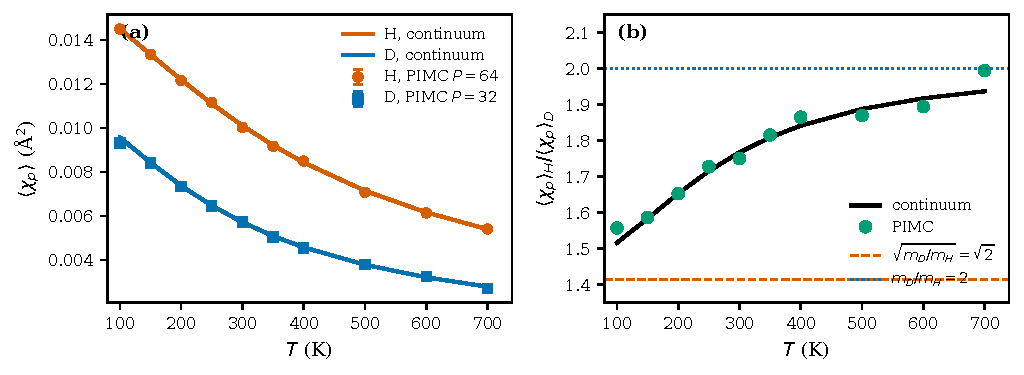
\includegraphics[width=0.95\textwidth]{../figures/fig2_harmonic.pdf}
\caption{\label{fig:harmonic}
Harmonic path spread for $\omega=1000\,\mathrm{cm}^{-1}$.
(a)~$\avg{\chip}(T)$ from Eq.~\eqref{eq:chip_harm} (lines) and Levy-staging PIMC (symbols).
(b)~Isotope ratio, with the $T\to 0$ limit $\sqrt{2}$ and the $T\to\infty$ limit $2$.
(c)~Bead convergence of $\avg{\chip}_H$ at $300\,\mathrm{K}$: PIMC versus the exact finite-$P$ formula, Eq.~\eqref{eq:chip_P}.
}
\end{figure*}

\subsection{Eckart barrier}

The symmetric Eckart barrier with width $a=0.50\,\text{\AA}$ provides thermal rates that do not depend on path-integral sampling. Figure~\ref{fig:eckart}(a) shows the exact tunneling correction $\kappa=k/k_{\mathrm{TST}}$ at $300\,\mathrm{K}$. For H, $\kappa$ increases from $1.28$ at $V_0=4\,\kB T$ to $2.68$ at $V_0=16\,\kB T$; the corresponding Wigner factors are $1.22$ and $1.86$. Wigner is therefore a useful first correction at moderate $\hbar\omega_b/\kB T$ and underestimates the exact $\kappa$ once $\hbar\omega_b/\kB T\gtrsim 4$. Deuterium remains closer to TST, as expected from the lower barrier frequency.

The exact KIE [Fig.~\ref{fig:eckart}(b) and Table~\ref{tab:eckart}] is $1.68$ at $4\,\kB T$ and $2.28$ at $16\,\kB T$. Classical TST contributes only $\sqrt{m_D/m_H}=\sqrt{2}\approx 1.414$, independent of barrier height. The Wigner KIE tracks the exact result qualitatively ($1.55$ to $1.84$) but lags at the highest barriers. These numbers set the scale of the nuclear quantum effect that a path-spread diagnostic is meant to resolve. They are \emph{not} QRR rates: the Eckart calculation is exact one-dimensional scattering, used here as an independent benchmark of when tunneling matters.

\begin{table}[htbp]
\caption{\label{tab:eckart}
Symmetric Eckart barrier at $T=300\,\mathrm{K}$, $a=0.50\,\text{\AA}$.
$\kappa=k/k_{\mathrm{TST}}$.
Classical KIE is $\sqrt{2}$ at every barrier.
}
\begin{ruledtabular}
\begin{tabular}{lccccc}
$V_0/\kB T$ & $\hbar\omega_b^H/\kB T$ & $\kappa_H$ & $\kappa_D$ & KIE (exact) & KIE (Wigner) \\
\hline
$4$  & $2.27$ & $1.28$ & $1.08$ & $1.68$ & $1.55$ \\
$8$  & $3.22$ & $1.60$ & $1.28$ & $1.77$ & $1.67$ \\
$12$ & $3.94$ & $2.04$ & $1.36$ & $2.12$ & $1.76$ \\
$16$ & $4.55$ & $2.68$ & $1.66$ & $2.28$ & $1.84$ \\
\end{tabular}
\end{ruledtabular}
\end{table}

\begin{figure*}[t]
\centering
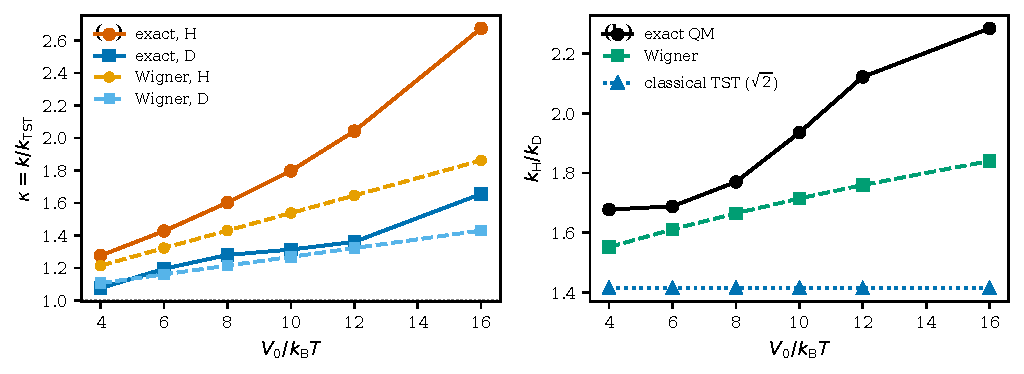
\includegraphics[width=0.95\textwidth]{../figures/fig4_eckart.pdf}
\caption{\label{fig:eckart}
Symmetric Eckart barrier, $a=0.50\,\text{\AA}$, $T=300\,\mathrm{K}$.
(a)~Exact and Wigner tunneling corrections versus barrier height.
(b)~Kinetic isotope effect. Classical TST is $\sqrt{2}$ at every $V_0$.
}
\end{figure*}

\subsection{Asymmetric double well}

The ADW $V(q)=V_0[(q/q_0)^2-1]^2+\alpha q$ with $q_0=0.70\,\text{\AA}$ is a bound proton-transfer model. Figure~\ref{fig:landscape}(a) shows the WHAM centroid PMF at $V_0=8\,\kB T$: the H barrier is $15.9\,\mathrm{kJ\,mol}^{-1}$ and the D barrier is $17.6\,\mathrm{kJ\,mol}^{-1}$. Figure~\ref{fig:landscape}(b) is the quantity QRR actually uses, the dividing-surface density $p^\ddagger(\chip)$. It is broader for H than for D, with means $\avg{\chip}_\ddagger^{\mathrm{H}}=0.015\,\text{\AA}^2$ and $\avg{\chip}_\ddagger^{\mathrm{D}}=0.008\,\text{\AA}^2$. With the bookkeeping cut $2\chi_c=0.020\,\text{\AA}^2$, the delocalized weight is $f_{\mathrm{deloc}}^{\mathrm{H}}=0.18$--$0.23$ across $V_0=2$--$8\,\kB T$, versus $f_{\mathrm{deloc}}^{\mathrm{D}}=0.014$--$0.045$ [Fig.~\ref{fig:landscape}(c) and Table~\ref{tab:adw}]. For H the fraction is essentially flat in this barrier window; the robust observation is the isotope contrast, not a strong barrier trend.

These are equilibrium path-class statistics, not rates. We do not convert $f_{\mathrm{deloc}}$ into a QRR rate or into a claimed improvement over RPMD. Two-dimensional histograms of $F(\xip,\chip)$ from the same umbrellas are too sparsely sampled in $\chip$ to publish as free-energy surfaces.

\begin{table}[htbp]
\caption{\label{tab:adw}
Asymmetric double well at $T=300\,\mathrm{K}$.
Centroid barriers from 1D WHAM; $f_{\mathrm{deloc}}$ from the WHAM-weighted dividing-surface ensemble with $2\chi_c=0.020\,\text{\AA}^2$.
}
\begin{ruledtabular}
\begin{tabular}{lcccccc}
$V_0/\kB T$ & $\Delta F_H$ & $\Delta F_D$ & $f_{\mathrm{deloc}}^H$ & $f_{\mathrm{deloc}}^D$ & $\avg{\chip}_\ddagger^H$ & $\avg{\chip}_\ddagger^D$ \\
 & (kJ/mol) & (kJ/mol) & & & (\AA$^2$) & (\AA$^2$) \\
\hline
$2$ & $4.25$ & $4.60$ & $0.18$ & $0.014$ & $0.014$ & $0.007$ \\
$4$ & $8.90$ & $9.02$ & $0.23$ & $0.020$ & $0.015$ & $0.007$ \\
$6$ & $12.4$ & $14.3$ & $0.22$ & $0.024$ & $0.015$ & $0.007$ \\
$8$ & $15.9$ & $17.6$ & $0.23$ & $0.045$ & $0.015$ & $0.008$ \\
\end{tabular}
\end{ruledtabular}
\end{table}

\begin{figure*}[t]
\centering
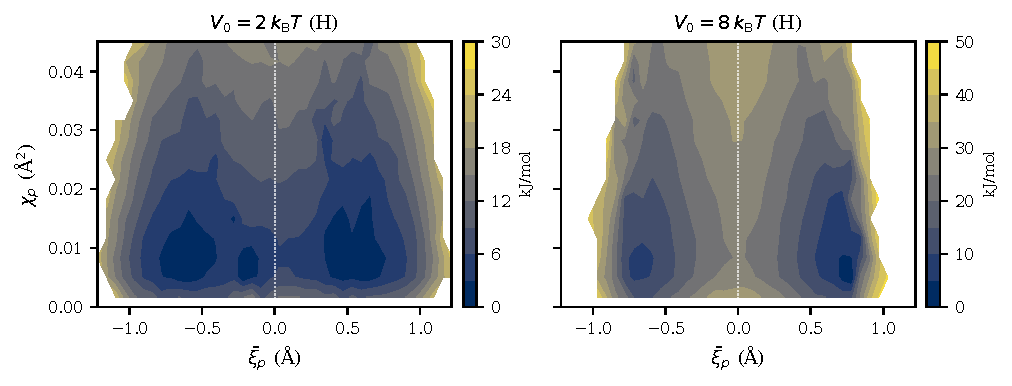
\includegraphics[width=0.95\textwidth]{../figures/fig5_landscape.pdf}
\caption{\label{fig:landscape}
Asymmetric double well, $T=300\,\mathrm{K}$.
(a)~Centroid PMF at $V_0=8\,\kB T$.
(b)~Dividing-surface path-spread density $p^\ddagger(\chip)$ at the same barrier; the dotted line is the bookkeeping cut $2\chi_c$.
(c)~Delocalized fraction versus barrier height. The H fraction is nearly flat; the D fraction remains an order of magnitude smaller.
}
\end{figure*}

\subsection{What is not shown}

A bilinear proton--solvent model $V=V_{\mathrm{ADW}}(q_p)+\tfrac12 k_s q_s^2+\kappa_c q_p q_s$ was sampled without umbrellas. Dividing-surface correlations $\mathrm{corr}(\chip,q_s)$ lie between $-0.06$ and $-0.16$ with a few hundred crossings and do not trend cleanly with $\kappa_c$. That scan is not evidence for or against Proposition~\ref{prop:factorize}; a controlled test would require umbrella sampling in $(\xip,\chip,\lambda_s)$. We therefore omit it from the figures.

\section{Discussion}
\label{sec:discussion}

QRR does not replace RPMD, instanton theory, or vibronic PCET rate laws.\cite{craig2005,richardson2018,soudackov2000,goldsmith2019} RPMD remains the appropriate dynamical correction to centroid QTST in the crossover regime; instanton theory remains the appropriate semiclassical description when a single tunneling orbit dominates; Hammes--Schiffer vibronic theory remains the appropriate nonadiabatic framework when electron-proton nonadiabaticity is essential. What $\chip$ adds is an equilibrium resolution of imaginary-time geometries that those methods otherwise average or optimize.

The present calculations do not evaluate Eq.~\eqref{eq:kQRR} as a rate. Doing so would require a class-conditional transmission coefficient, which we have not computed. The Eckart section reports exact scattering rates; the ADW section reports $p^\ddagger(\chip)$. Connecting the two is an analogy, not a numerical identity.

Two condensed-phase hypotheses follow, and should be treated as such. First, if an increase of the observed KIE with driving force\cite{goldsmith2019,koper2011} is carried by tunneling-like paths, $\Delta f_{\mathrm{deloc}}=f_{\mathrm{deloc}}^{\mathrm{H}}-f_{\mathrm{deloc}}^{\mathrm{D}}$ should increase with that driving force. Second, a breakdown of $F=F_p+F_s$ at the dividing surface would be a signature of proton--solvent coupling beyond a product Marcus picture. Neither hypothesis is tested here.

Limitations are sharp. $\chip$ is an imaginary-time polymer statistic, not a spectroscopic observable. The cut $\chi_c$ is bookkeeping; Fig.~\ref{fig:landscape}(b) is the primary object. Recrossing is not resolved by class. The models are one-dimensional. Finite-$P$ errors in $\chip$ are under control for the $1000\,\mathrm{cm}^{-1}$ mode at $P\ge 32$; stiffer stretches will need more beads or a virial estimator.

\section{Conclusions}

We have defined a projected ring-polymer path spread $\chip$ for proton transfer, derived its harmonic continuum and finite-bead limits, and used it to resolve the centroid dividing-surface ensemble. Levy-staging Monte Carlo reproduces the exact finite-bead harmonic formula to about one percent. Exact Eckart rates quantify when tunneling corrections and KIEs depart from TST. On an asymmetric double well, the dividing-surface path-spread distribution is robustly broader for H than for D. Equation~\eqref{eq:kQRR} is a bookkeeping decomposition of QTST; it is not shown here to be a better rate. The estimator is a collective variable and can be accumulated in any path-integral molecular dynamics run.

\begin{acknowledgments}
Computational work was performed on local workstations. No external funding is declared.
\end{acknowledgments}

\section*{Data Availability Statement}
The data that support the findings of this study are openly available in Zenodo at \url{https://doi.org/10.5281/zenodo.22718950} (Ref.~\onlinecite{vubangsi2026zenodo}).
The source repository is \url{https://github.com/vmercel/QRR-PCET}.

\bibliographystyle{aipnum4-2}
\bibliography{../references/references}

\end{document}
